% Chapter 2 — Context & Background

\chapter{Context \& Background}

\label{Chapter2}

\section{Operating Principle of a PEM Fuel Cell}

A proton exchange membrane fuel cell (PEMFC) converts the chemical energy of
hydrogen and oxygen directly into electricity, heat, and water
\cite{manana2006,mohiuddin2018,thomya2011}. At the anode, hydrogen splits into
protons and electrons. The protons cross the polymer membrane, while the
electrons travel through the external circuit and supply the load. At the
cathode, oxygen recombines with both to form water (Figure~\ref{fig:pemfc-operation}).
The overall reaction is
\begin{equation*}
    \mathrm{H_2 + \tfrac{1}{2}O_2 \rightarrow H_2O + electricity + heat}.
\end{equation*}
The membrane conducts protons, blocks electrons, and separates fuel from
oxidant. Together with the two electrodes it forms the membrane electrode
assembly (MEA), the elementary repeating unit of the stack
\cite{manana2006,ionescu2020}. Water management is critical to performance: a dry
membrane loses proton conductivity, whereas excess liquid water floods the gas
channels. Stable operation therefore requires a balance between hydration and
drainage \cite{weber2004,zhang2017}.

\begin{figure}[t]
    \centering
    \begin{subfigure}[t]{0.56\linewidth}
        \centering
        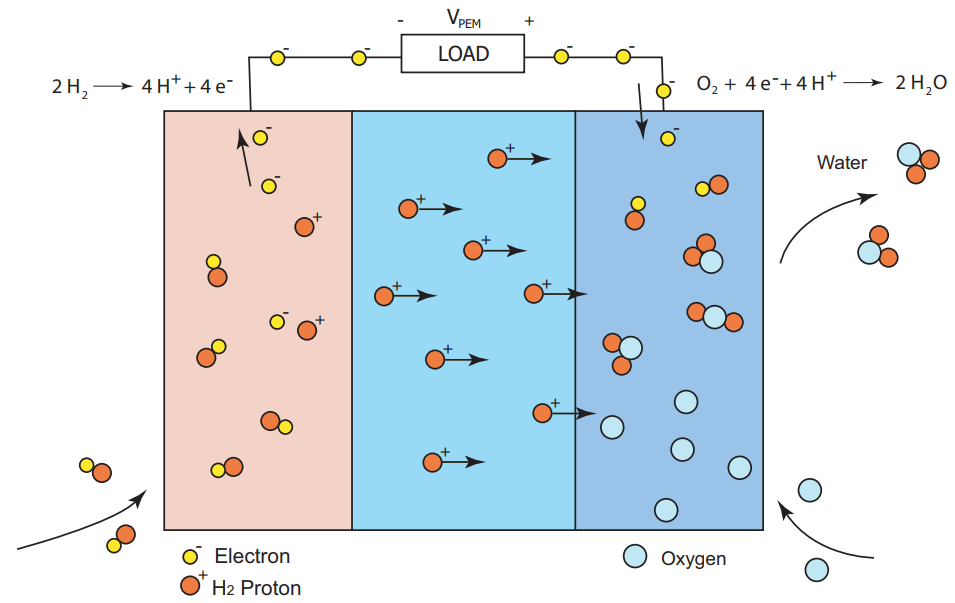
\includegraphics[width=\linewidth]{Figures/pemfc_operation.png}
        \caption{Electrochemical operation: hydrogen oxidation at the anode,
                 proton transport through the membrane, oxygen reduction at the
                 cathode.}
    \end{subfigure}
    \hfill
    \begin{subfigure}[t]{0.38\linewidth}
        \centering
        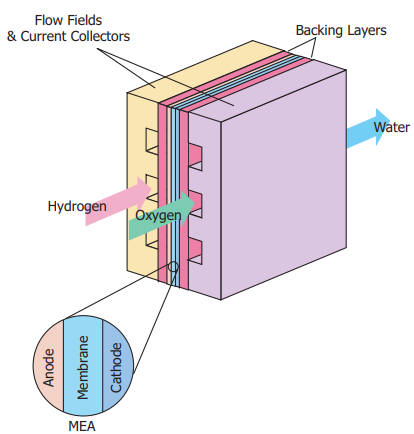
\includegraphics[width=\linewidth]{Figures/pemfc_stack_structure.png}
        \caption{Stack structure: individual MEAs stacked in series to add their
                 voltages.}
    \end{subfigure}
    \caption[Operating principle and structure of a PEM fuel cell]{Operating
             principle and physical structure of a PEM fuel cell. A single cell
             delivers roughly one volt, so cells are stacked in series to reach a
             useful voltage \cite{mohiuddin2018,thomya2011,manana2006}.}
    \label{fig:pemfc-operation}
\end{figure}

\section{Voltage Losses and Polarization Behavior}

A practical cell delivers less than its reversible (open-circuit) voltage because
of three loss mechanisms, each dominant in a different region of the polarization
curve (Figure~\ref{fig:pemfc-losses}) \cite{manana2006,pukrushpan2003,thanapalan2008}:
\begin{itemize}
    \item \textbf{activation loss} --- the kinetic penalty of driving the
          electrode reactions, dominant at low current \cite{pukrushpan2003,weber2004};
    \item \textbf{ohmic loss} --- the resistive drop across the membrane and
          conductors, approximately linear in current \cite{pukrushpan2003,thanapalan2008};
    \item \textbf{concentration loss} --- the mass-transport limitation that
          causes the steep voltage drop at high current \cite{manana2006,weber2004}.
\end{itemize}
The \emph{polarization curve} is the cell voltage plotted against current density;
it is the fingerprint of cell performance and the basis for the model of
Chapter~\ref{Chapter3}. Fast transients are further shaped by the charge
double-layer at the electrode/electrolyte interface, which behaves as a small
capacitor in equivalent-circuit models \cite{pukrushpan2003,manana2006}.

\begin{figure}[t]
    \centering
    \begin{subfigure}[t]{0.48\linewidth}
        \centering
        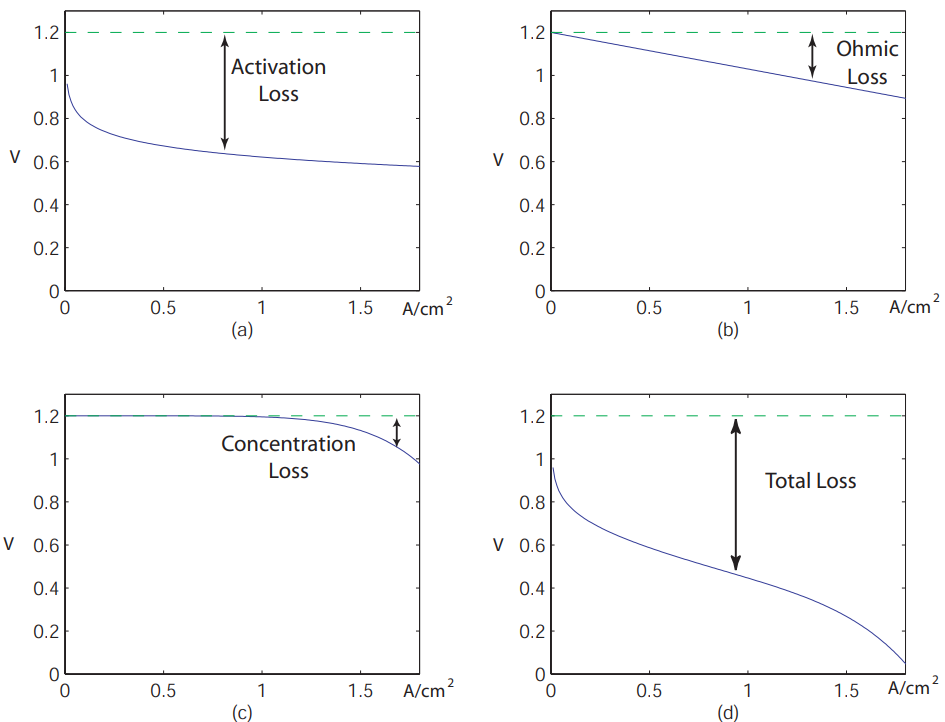
\includegraphics[width=\linewidth]{Figures/pemfc_loss_components.png}
        \caption{Decomposition into activation, ohmic, and concentration losses.}
    \end{subfigure}
    \hfill
    \begin{subfigure}[t]{0.48\linewidth}
        \centering
        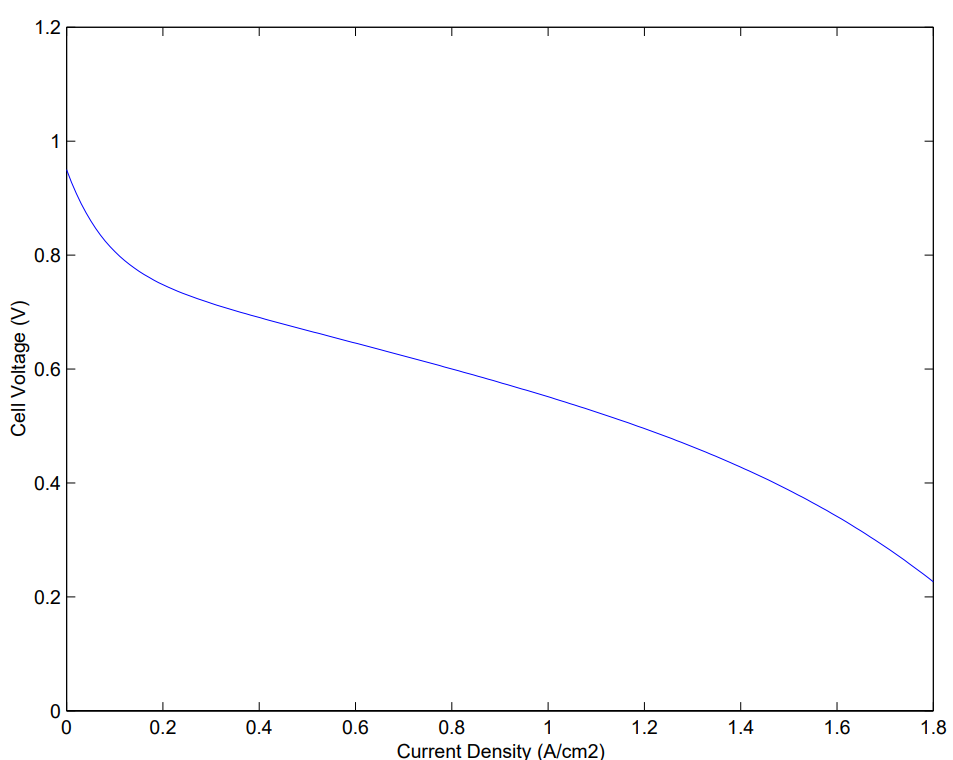
\includegraphics[width=\linewidth]{Figures/pemfc_polarization_curve.png}
        \caption{Resulting polarization curve.}
    \end{subfigure}
    \caption[Voltage losses and polarization curve]{Influence of the three loss
             mechanisms on PEMFC performance. Activation dominates at low current,
             ohmic loss in the middle, and concentration loss near the limiting
             current --- together they bend the ideal flat voltage into the
             characteristic polarization curve.}
    \label{fig:pemfc-losses}
\end{figure}

\section{State of the Art}
\label{sec:sota}

Control-oriented PEMFC modeling traces back to the system-level model of
Pukrushpan \cite{pukrushpan2003}, which couples a polarization-curve voltage law
with compressor, manifold-filling, and membrane-hydration dynamics; most later
models specialize or simplify it \cite{thanapalan2008,kim2010,zhu2017}. Simplified
electrical models reproduce the static voltage--current characteristic of small
stacks with only a handful of parameters \cite{manana2006,shen2005}. Crucially,
per-cell measurements on a small stack reveal voltage deviations of up to 7\,\%
between cells \cite{manana2006}, which motivates the per-cell calibration adopted
here. Parameter identification by direct-search optimization on measured voltage
and power was formalized by Thanapalan et al.\ \cite{thanapalan2008} and extended
with modern metaheuristics \cite{cao2019}.

On the control side, proportional--integral (PI) regulation of flows, pressures,
and converter currents is the established baseline \cite{zhu2017,derbeli2017}.
Documented upgrades include linear-quadratic (LQ) multivariable control,
time-delay control, and model-predictive schemes
\cite{pukrushpan2003,kim2010,wang2021simulation}. At system level, the response
delays of the air and hydrogen supply components remain the main factor limiting
dynamic operation \cite{kharrat2025}.

\subsection{Practical Challenges and Choice of Control Strategy}
\label{sec:challenges}

The control strategy of this work was shaped directly by constraints observed on
the laboratory bench. The most natural actuator for a fuel cell is the hydrogen
supply: raising the anode pressure raises the Nernst voltage and the available
current. In practice, however, the usable hydrogen pressure on the educational
stack is narrowly bounded. The supply regulator caps the inlet pressure, and a
large anode--cathode pressure difference risks mechanical damage to the thin
membrane \cite{zhu2017,kharrat2025}. The pressure can therefore be varied only
within a small range, which yields too little authority to regulate the operating
point across the full load. Direct current control through the hydrogen valve was
explored and found impractical for the same reason: the actuator saturates before
the load demand is met.

This limitation motivated the chosen approach. Rather than acting on the slow,
saturation-limited gas supply, the control is moved to the electrical side: the
stack feeds a DC/DC boost converter whose duty cycle is set by a fast PI loop
\cite{derbeli2017}. The converter decouples the load from the cell and shapes the
delivered power, while the hydrogen supply is left to maintain an adequate
pressure rather than to track the load. This separation of roles --- electrical
control for the fast dynamics, gas supply for the slow operating conditions ---
underlies the architecture developed in Chapter~\ref{Chapter5}.
